\section{AI model in production}

Deploying a predictive models into production is quite complex. Choosing how to putting models into productions which can depend on the specific use case. A good summary of different deployment approaches has been described in \cite{deploying-ML}. This section only show a simple example on how to save and load a pre-trained model for production.  

\subsection{From model to production}

Data scientists/engineer often do their prototype application in Jupyter Notebooks \cite{Jupyter-Notebooks}.
An ad-hoc trained model in Jupyter can be pushed to production with different types of libraries and other notebook providers. 

The model can be save in different format:

\begin{itemize}
    \item \textbf{Pickle} converts a python object to to a bitstream and allows it to be stored to disk and reloaded at a later time \cite{ML_Apporaches}.
    \item \textbf{ONNX} the Open Neural Network Exchange format, is an open format that supports the storing and porting of predictive model across libraries and languages. Most deep learning libraries support it and sklearn \cite{scikit-learn} also has a library extension to convert their model to ONNX’s format \cite{ML_Apporaches}.
    \item \textbf{PMML} or predictive model markup language, is another interchange format for predictive models. Like for ONNX sklearn also has another library extension for converting the models to PMML format. It has the drawback however of only supporting certain type of prediction models.PMML has been around since 1997 and so has a large footprint of applications leveraging the format. Applications such as SAP for instance is able to leverage certain versions of the PMML standard, likewise for CRM applications such as PEGA \cite{ML_Apporaches}.
    \item \textbf{POJO and MOJO} are H2O.ai’s export format, that intendeds to offers an easily embeddable model into java application. They are however very specific to using the H2O’s platform \cite{ML_Apporaches}.
\end{itemize}

\subsection{Save and Load the model}

Python pickle module is one of the most popular object serialization packages. It serializes objects so they can be saved to a file, and loaded in a program again later on. 

Datacamp website give a good explanation on Pickle in Python, when (not) to use it, how to compress pickled objects, multiprocessing \cite{Pickle}

In figure \ref{figure:scikitpickle} the scikitlearn model can be saved and loaded with a few lines of code.

\begin{figure}[H]
	\centering
	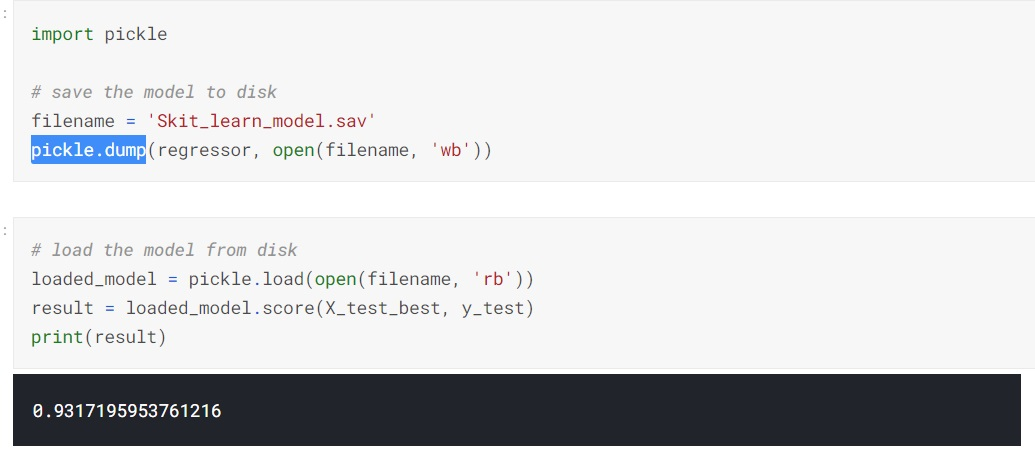
\includegraphics[width=0.8\columnwidth]{Pictures/scikitlearn_pickel.jpg}
	\caption[Short title]{Save and Load scikit learn model with pickle}
	\label{figure:scikitpickle}
\end{figure}

The model also can be trained with "GPU" to accelerate the training process and load with "CPU" later to save the memory.

In figure \ref{figure:savetorch} and \ref{figure:loadtorch} the model had been trained with GPU and later load in CPU using pytorch libraries. 

\begin{figure}[H]
	\centering
	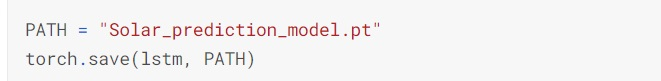
\includegraphics[width=0.8\columnwidth]{Pictures/save_LSTM.jpg}
	\caption[Short title]{Save Pytorch model}
	\label{figure:savetorch}
\end{figure}

\begin{figure}[H]
	\centering
	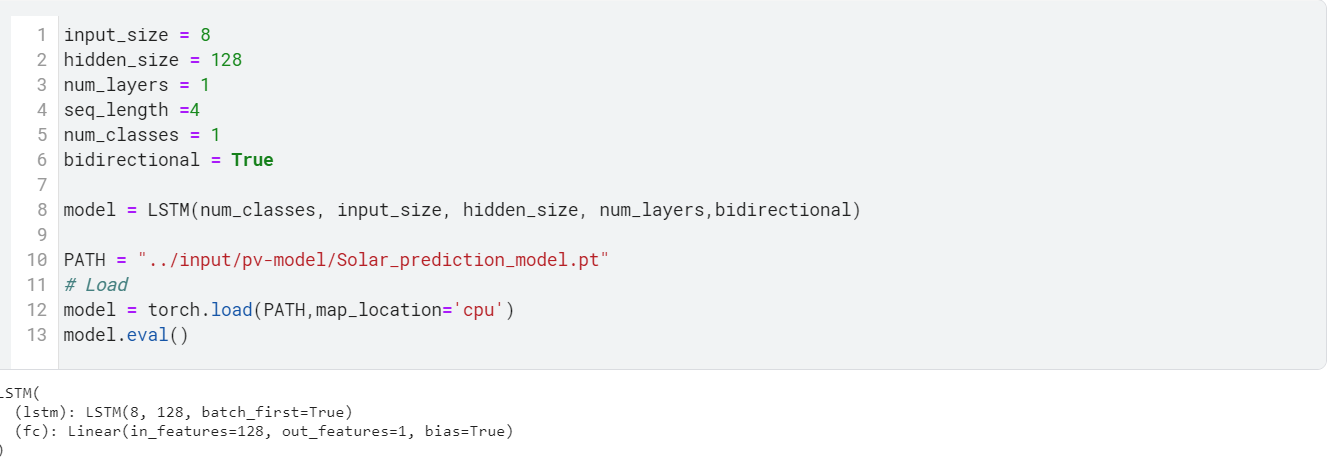
\includegraphics[width=0.8\columnwidth]{Pictures/load lstm.png}
	\caption[Short title]{Load Pytorch model}
	\label{figure:loadtorch}
\end{figure}

\newpage